\documentclass[letterpaper,11pt]{article}

\usepackage{graphicx}
\usepackage{multicol}
\usepackage{fullpage}
\usepackage[margin=0.5in,letterpaper]{geometry}
\setlength{\footskip}{15pt}
\usepackage{floatflt}
\usepackage{xspace}
\linespread{0.95}
\def\degC{$^{\circ}$C }
\def\degf{$^{\circ}$F }
\def\vol #1 {{\bf #1}, $\;\;$}
\def\refer{\par\noindent\hangindent\parindent\hangafter1}


\title{\vspace{-2.0cm}Herzmann Family Christmas Letter 2017}
\author{Daryl Herzmann${}^1$, Elizabeth Herzmann${}^1$, Margaret 
Herzmann${}^2$,\\
Robert Herzmann${}^3$, AND Charlotte Herzmann${}^4$ \\
\it{${}^1$ Caretakers},
\it{${}^2$ Senior Child},
\it{${}^3$ Stinker},
\it{${}^4$ Final Child}}
\date{15 December 2017}

\makeatletter
\newenvironment{tablehere}
  {\def\@captype{table}}
  {}

\newenvironment{figurehere}
  {\def\@captype{figure}}
  {}
\makeatother

\newcommand{\Line}[0]{%
  \rule{0cm}{0cm}\\\hrule\rule{0cm}{0cm}%
}

%\addtolength{\textheight}{1.5in}

\begin{document}
\maketitle
\vspace{-0.75cm}
\begin{abstract}
Concerns have been raised over the efficacy of this letter. For assessment
purposes, an external review committee was empaneled.  Panelists reviewed the
previous four letters and expressed concerns over \textbf{i)} spelling mistakes
and \textbf{ii)} busted forecasts.  The committee was thanked for their work and
their recommendations were later ignored.  To address readership and retention,
a ploy used by the author's childhood Rural Electric Cooperative (REC) was to
embed customer's account numbers within the text of the monthly newsletter.  If
you spotted your number, you could redeem a bill credit.  For the context of this
letter, seeing your street addresses yields an Amazon Gift Card.
\end{abstract}

\vspace{-0.5cm}
\Line
%\vspace{-0.5cm}

\begin{multicols}{2}

\section{Introduction} 

Last year's letter (Herzmann et al, 2016) contained a prognostication of an
arrival date of Baby Charlotte on 17 Jan 2017.  For tax benefit purposes, the
decision was made to have the child three weeks early during 2016. More on this
decision can be in Section 2. Our family now comprises Daryl "Daryl" (39),
Elizabeth "Liz"[not known to be pregnant] (33), Margaret "Miss Maggie" (4),
Robert "Ro-Ro" (3), Charlotte [no established nickname yet] (0), and one
tempormental cat named Snoopy (9).

\subsection{Housing}

No changes have been made with our housing arrangement. You should continue
to locally denote our snail mail address in permanent marker. The only project
of significance was the construction of a 4.5 \SI{10}{m^{2}} sandbox. Over 1.4
\mathrm{t} of sand was used to fill the box.  Each child has sufficient space to
violently swing objects without fear of hitting another child and/or
participating parent.

\subsection{Conveyances}

Again, last year's letter (Herzmann et al, 2016) contained a busted forecast
about Daryl requiring a minivan to schlepp the growing family around suburban
Des Moines. (A miracle occurred) and a different vehicle was not required.

\subsection{Employment}
Daryl remains gainfully employed by Iowa State University and continues to
work in disclipines foreign to the current US President's Administration, like
science, climate change, and common sense.

\begin{figurehere}
 \centering   
 \resizebox{.95\columnwidth}{!}{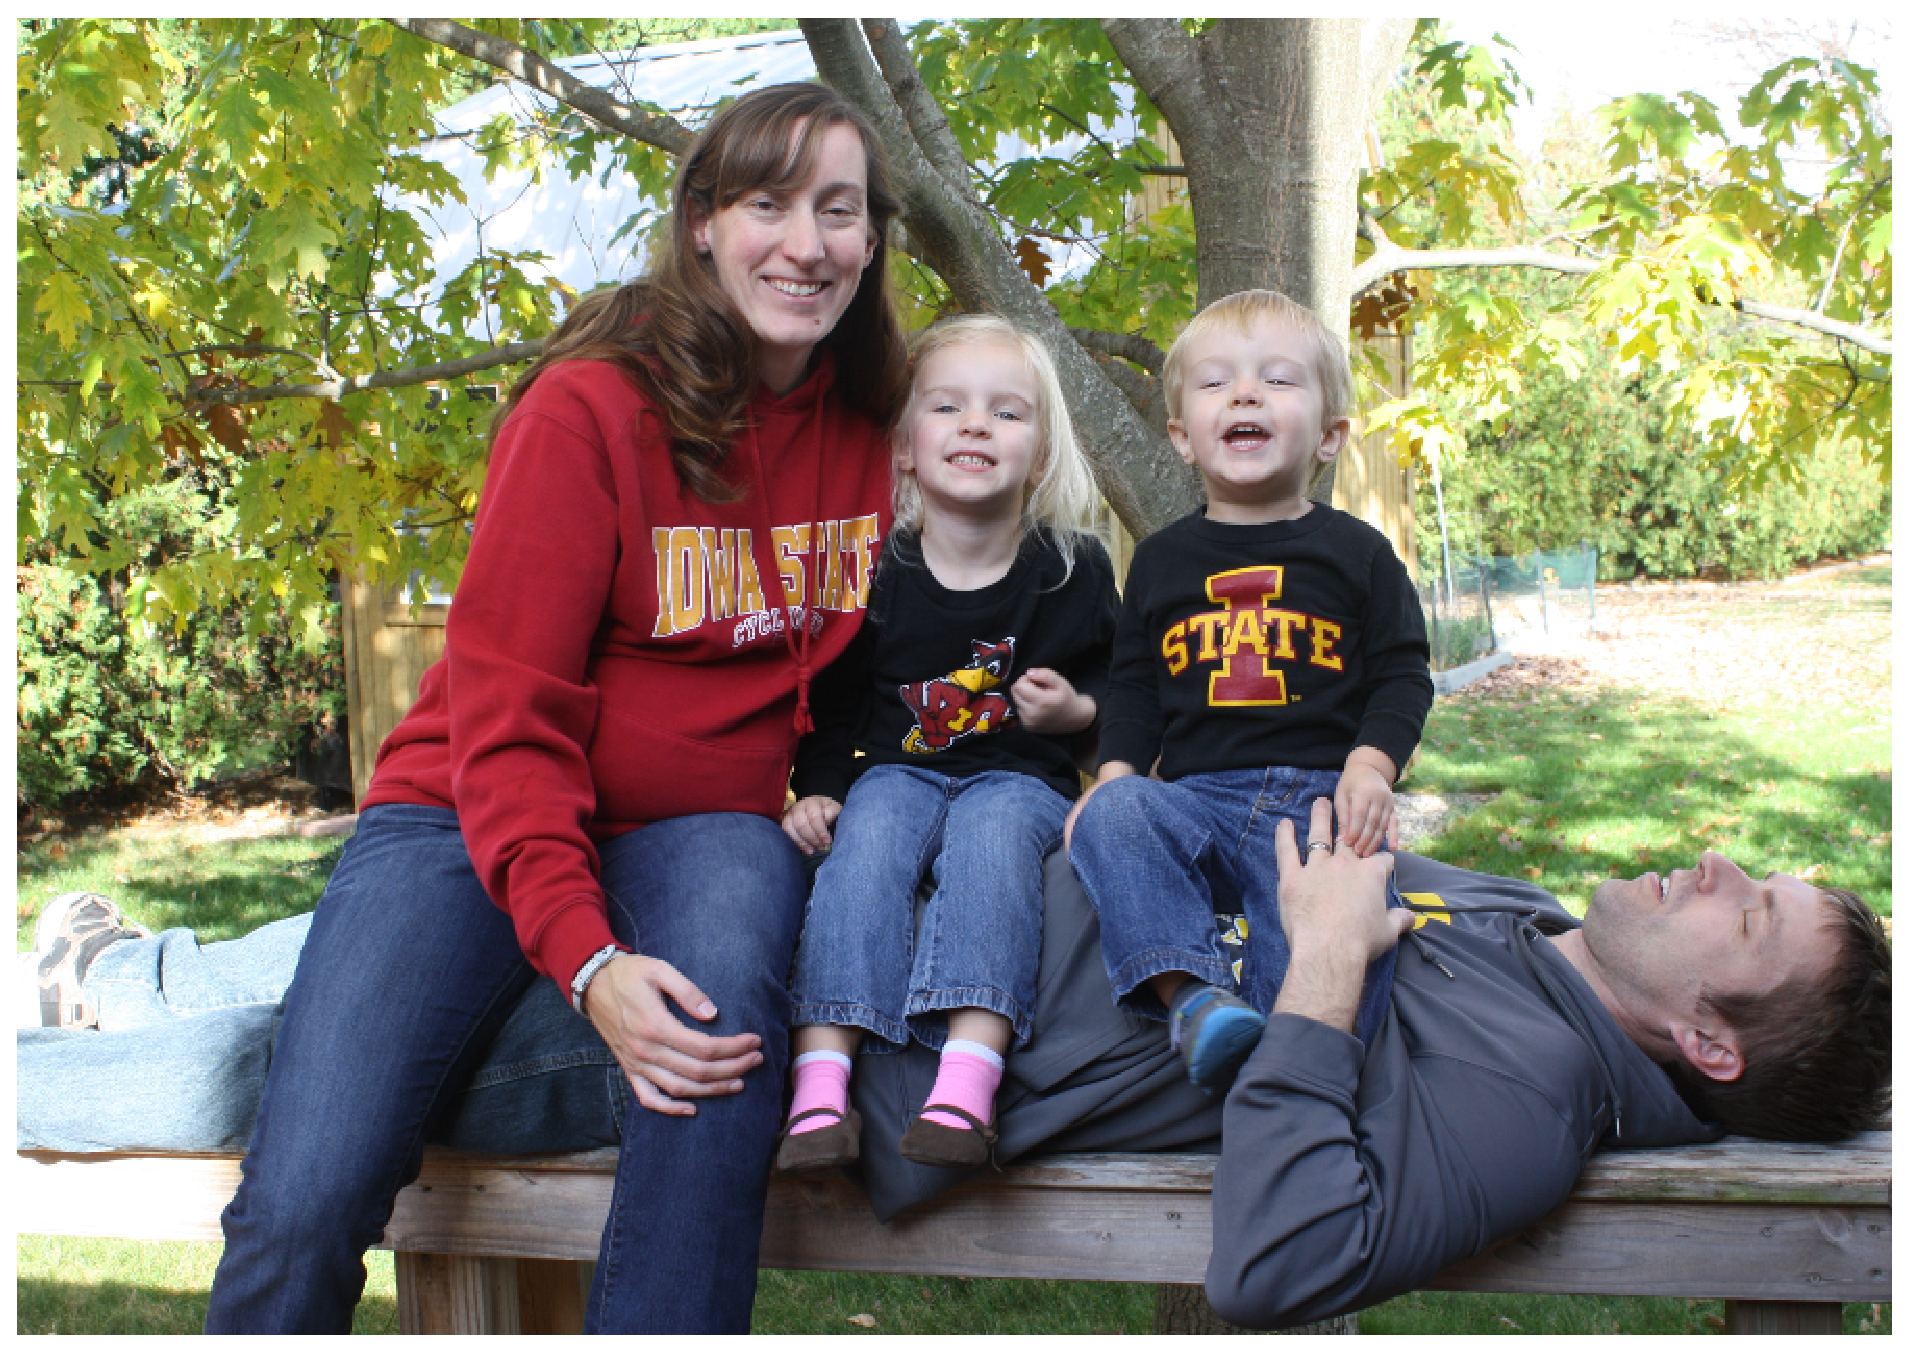
\includegraphics[angle=0]{plots/f1_2016.eps}}
 \caption{Representative depiction of Daryl's support of the growing family.}
\end{figurehere}

Liz continues her work at Johnston Middle School with 8th and 9th graders. 
The Science Olympiad program, which Liz coaches, continues to flourish. 
This year, she moved her classroom into the remodelled former High School.  The
new paint was barely dry and the room lights were installed the day before the
first day of class.

Miss Maggie and Mr Robert both have chores that they should be doing.  Miss
Charlotte is a free loader for now.

\section{Miss Charlotte}

Our latest arrival, arrived three weeks early on 28 Dec 2016.  From Daryl's
perspective, the labour and birth were both much more difficult and took longer
than the previous children.  Being early and a difficult birth likely both
conspired to place Charlotte in the NICU for the first week of her life.  Our
family is so thankful for the excellent care at the hospitol and tremendous
support we received from our family and friends.  Daryl particularly enjoyed the
near endless train of good food that arrived at our door during the period.

Miss Charlotte has since grown a lot and now easily walks wherever she wants to
go. The previously two children were laggards in this area.  However,
Miss Charlotte has not said any words yet, whereas the other children had by
this age.  For a good while this year, Miss Charlotte struggled sleeping. 
Figure 2 provides a summary of sleep quality for each member of our family.

\bigskip

\begin{figurehere}
 \centering   
 \resizebox{.95\columnwidth}{!}{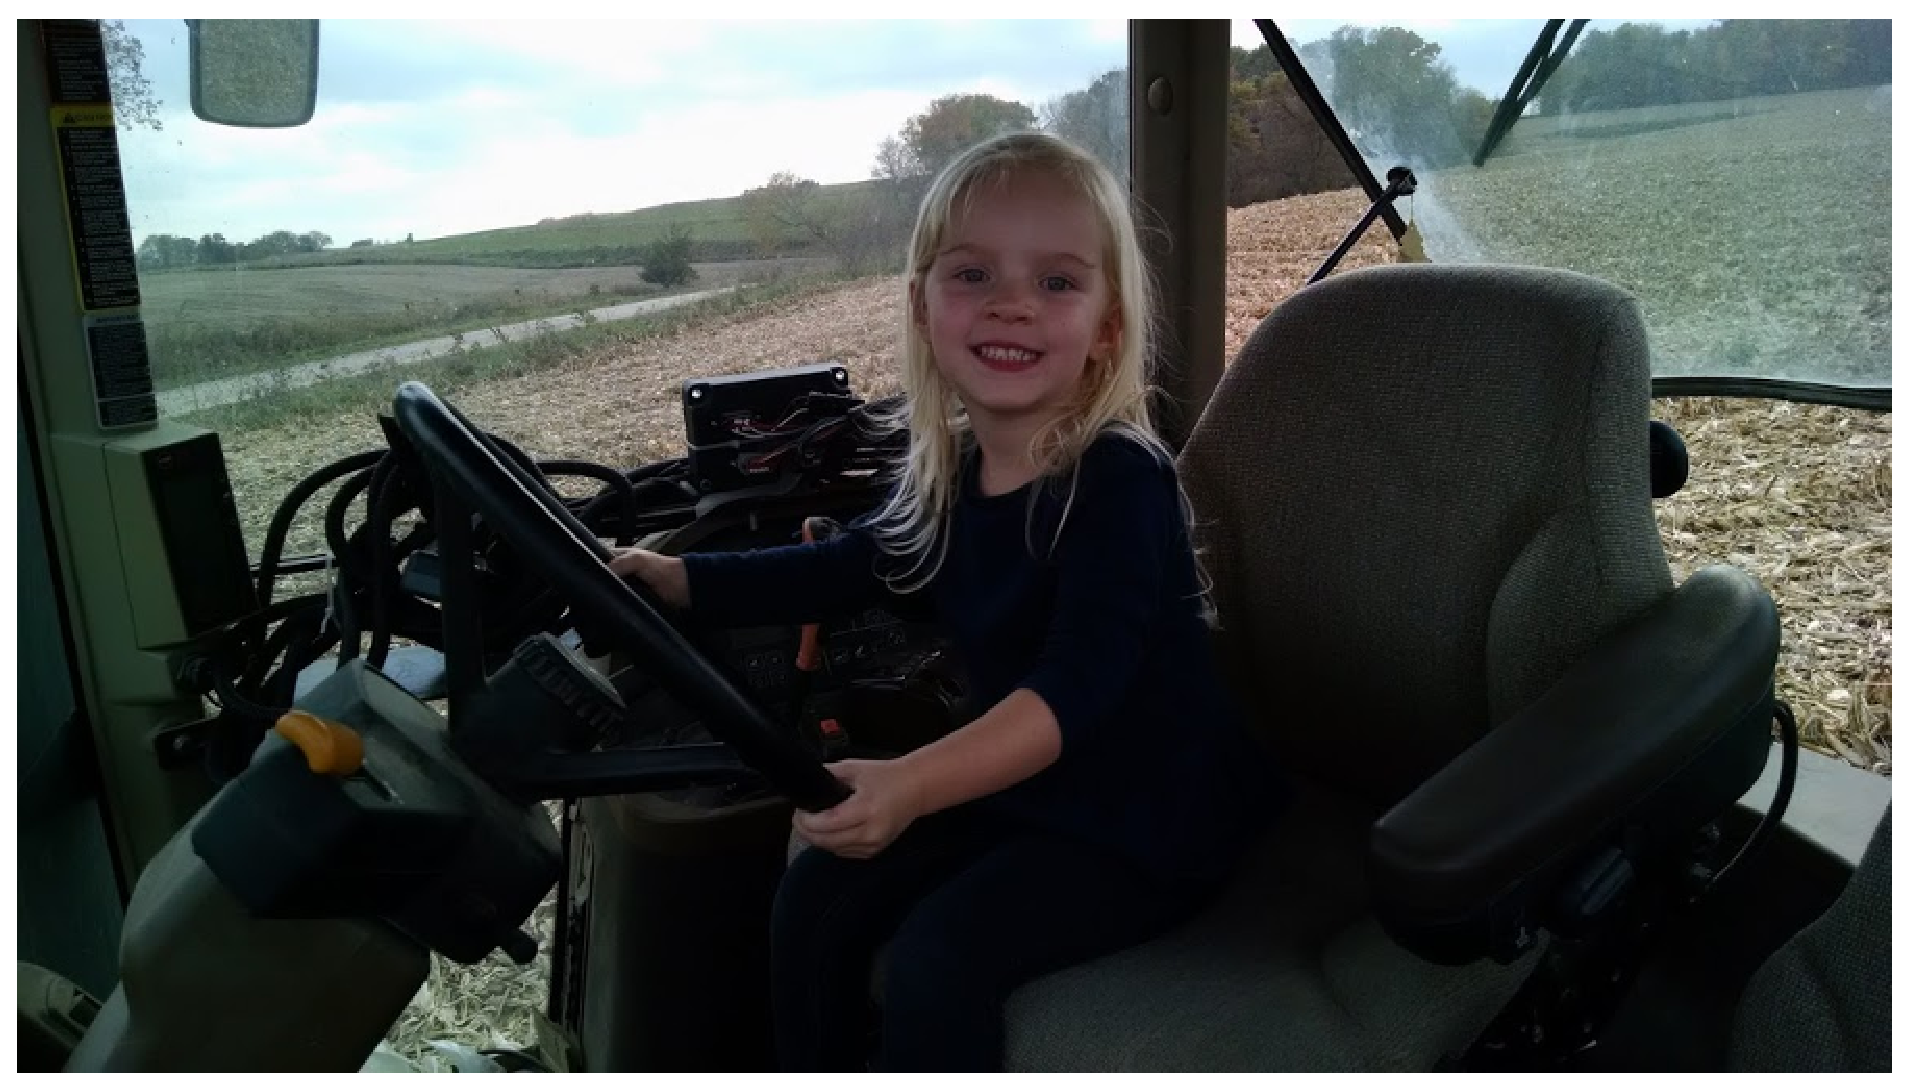
\includegraphics[angle=0]{plots/f3_2016.eps}}
 \caption{Miss Maggie safely driving her favorite tractor.}
\end{figurehere}

\section{Mr Robert}

Mr Robert is many handfuls of joy.  After the relative ease of raising Miss
Maggie, he has proven to be two orders of magnitude more challenging.  He now
shares a room with Miss Maggie and only recently has decided to sleep in his own
bed for the duration of the night. He seems to be an intelligent child, but has
a propensity of rearing back and raming his head into his unsuspecting parents. 

Mr Robert enjoys doing puzzles, eating pancakes or pizza, and wrestling with his
daddy after being told not to wrestle with pregnant mommy.  He is showing some
interest in potty training, but not ready to commit yet.

He is unsure about the arrival of Charlotte and after denoting the presence of a
baby in mommy's belly, he will left up his shirt to declare a baby in his belly
as well.  Once Charlotte gets bigger, he will move out of Maggie's room and back
into the nursery room with Charlotte joining Maggie.  Or maybe all three
children will be assigned to the same room to see what happens!

\section{Miss Maggie}

When not being fussy, Miss Maggie is mostly pleasant to deal with.  She is very
much excited about the arrival of Charlotte and wants to do most of the child
rearing herself. We just hope that Charlotte is not born on Miss Maggie's
birthday (13 January) as that may cause a change in her disposition.  Miss
Maggie loves to do art and mostly able to inscribe her name on paper and/or walls.

This fall, Miss Maggie went with her daddy to Grandma Barb's farm to help the
neighbors with the corn harvest.  She thought riding in the big green John Deere
tractor with a cab was the greatest thing ever (Figure 2).  Grandma Barb's
tractor (cabless) '\textit{does not have a door}', so Miss Maggie instructed her
to purchase a new tractor with a door.  She was a good helper for the brief
while at home and did not want to get out of the tractor. She threw a large fit
when asked to ride in a red colored tractor.

\section{Summary}

Our family continues to grow in size (Figure 3) and love (Figure 4). Thankfully
the increases in love are non-linear as each child has brought our family
infinite joy.  As long as there is two of everything in the house, the children
need not fight.  We hope Charlotte does not require purchasing three of
everything to keep the peace!

\begin{figurehere}
 \centering   
 \resizebox{.95\columnwidth}{!}{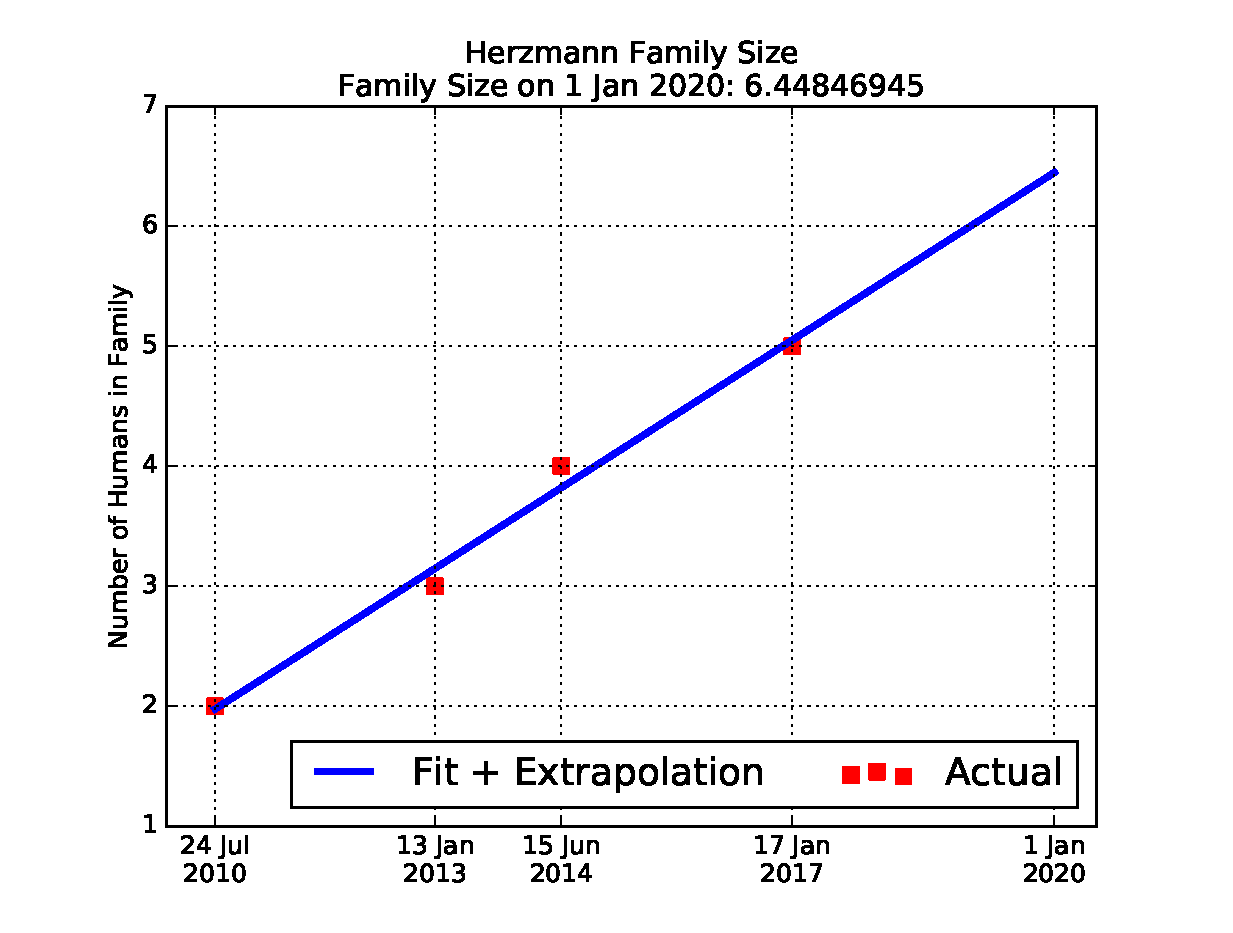
\includegraphics[angle=0]{plots/size.eps}}
 \caption{Actual and modeled family size.}
\end{figurehere}

\bigskip

\begin{figurehere}
 \centering   
 \resizebox{.95\columnwidth}{!}{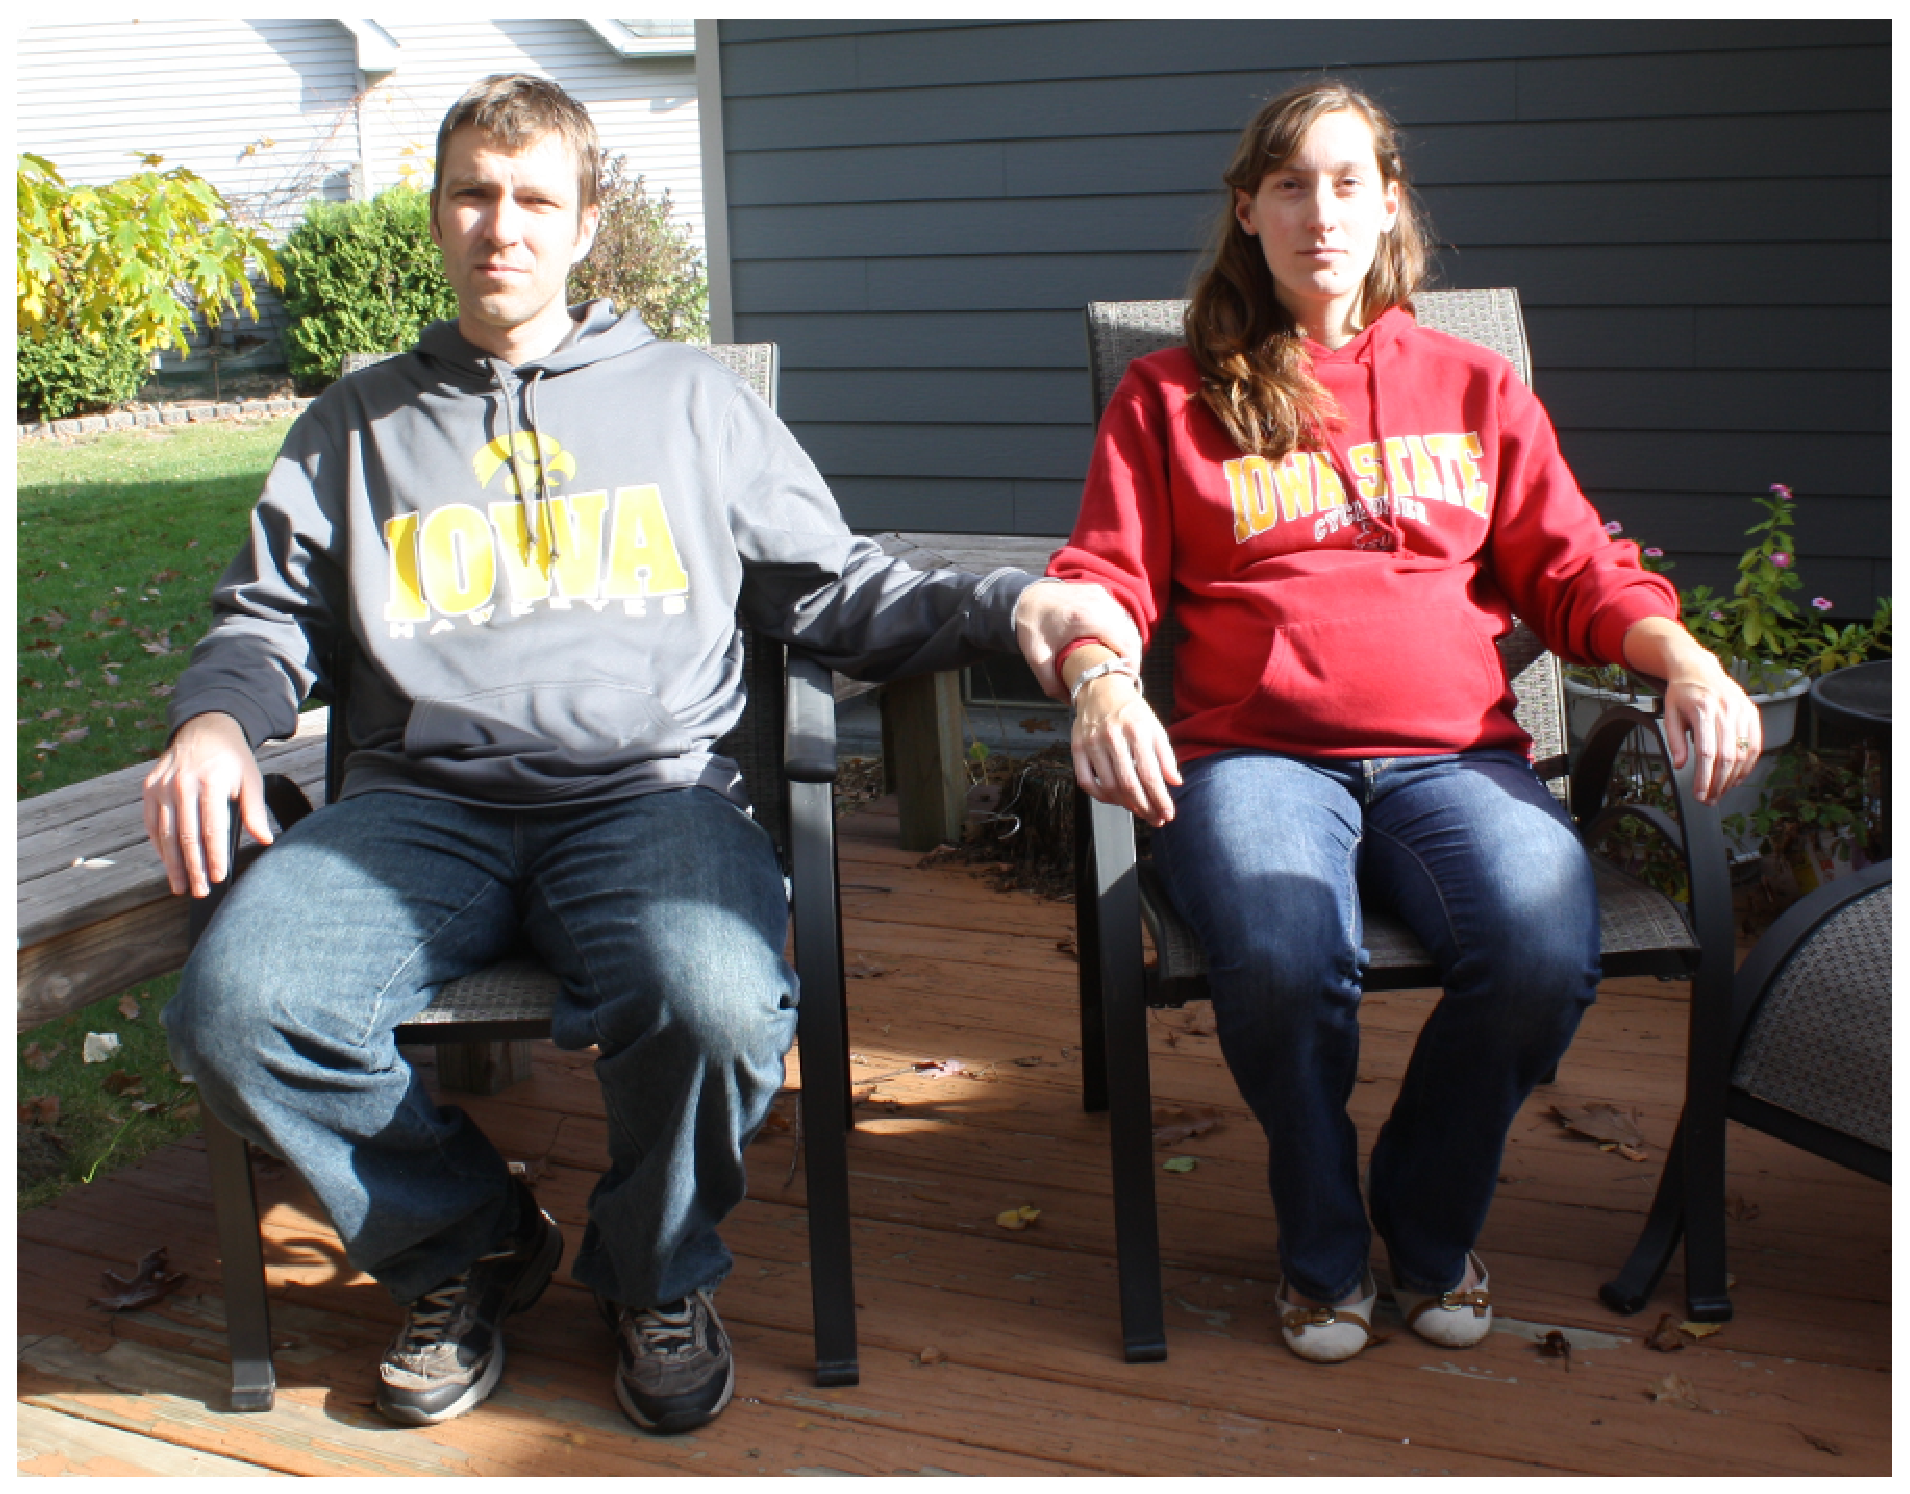
\includegraphics[angle=0]{plots/f2_2016.eps}}
 \caption{A candid and affectionate moment for a couple still very much in
 love.}
\end{figurehere}

\bigskip
  \emph{Acknowledgments} Our family wishes to thank you for the generous 
support, prayers, cards, gifts, and visits you have provided us in the past
year. With your continued support, this letter will be produced again
next year. Please note that the format chosen for this correspondence was
completely Daryl's idea and execution. Full \LaTeX\xspace source can be found on 
Daryl's Github page.

\section{References}

\refer Github, 2017: https://github.com/akrherz/me , visited 15 Dec 2017.
\refer Herzmann, Daryl E., et al. Herzmann Family Christmas Letter 2016. 

\end{multicols}

\end{document}

